\documentclass{article}
\usepackage[utf8]{inputenc}
\usepackage{graphicx}

\title{Informe Parcial II}
\author{daniel.perez19 }
\date{September 2021}

\begin{document}

\begin{titlepage}
    \begin{center}
        \vspace*{1cm}
            
        \Huge
        \textbf{Informe Parcial 2}
            
        \vspace{0.5cm}
        \LARGE
        Informática II
            
        \vspace{1.5cm}
            
        \textbf{Daniel Perez Gallego CC. 1193088770\\Jorge Montaña Cisneros CC.  1007327968}
            
        \vfill
            
        \vspace{0.8cm}
            
        \Large
        Departamento de Ingeniería Electrónica y Telecomunicaciones\\
        Universidad de Antioquia\\
        Medellín\\
        Septiembre de 2021
            
    \end{center}
\end{titlepage}

\tableofcontents

\section{Análisis del problema}
\subsection{Día 1}
Requerimos de una función para modificar el tamaño de las imagenes a un mismo valor, sin importar el tamaño orginal o de si sea menor a lo esperado.
Realizar una función para sacar todos los valores separados del RGB.
Segunda función será la altura en pixeles de nuestra imagen. Buscamos mas documentación para comprender más sobre el tema tratado.\\

Pensamos en una solución de separar las filas y columnas pares, dejando solamente las columnas pares, de este modo, tendremos la misma imagen, pero recortada a la mitad, luego realizamos el mismo proceso pero cortando las filas, obteniendo un tamaño menor pero proporcional a la imagen original, repiendo el proceso hasta obtener el tamaño deseado.\\

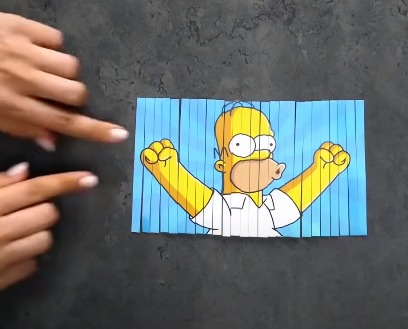
\includegraphics[width=4cm]{recorte1.jpeg}
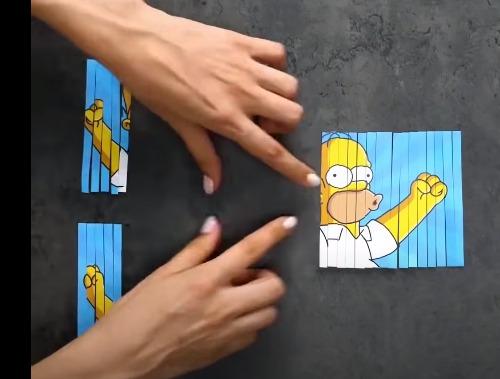
\includegraphics[width=4cm]{recorte2.jpeg}
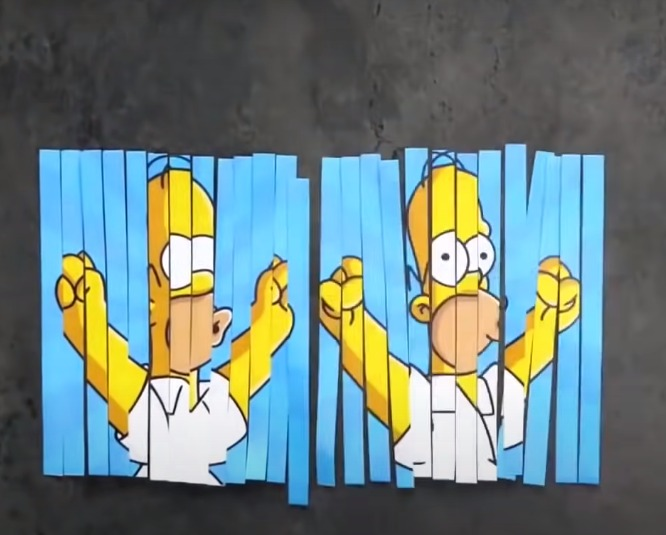
\includegraphics[width=4cm]{recorte3.jpeg}


\end{document}
